\section{Event generation and simulation details}
\label{sec:generation}

\subsection{Signal and background modelling}

Signal and background samples corresponding to $pp$ collisions at $\sqrt{s}=14$~TeV are generated using 
the {\sc Madgraph5} 2.1.1~\cite{Alwall:2011uj} leading-order (LO) generator and the  CTEQ6L1~\cite{Nadolsky:2008zw}  
set of parton distribution functions (PDF), interfaced to {\sc Pythia} v6.427~\cite{Sjostrand:2006za}  for parton 
showering and fragmentation and using the Perugia2011C~\cite{Skands:2010ak}  underlying event tune. In all cases, a top quark mass 
of 172 GeV is assumed and top quarks are decayed inclusively by {\sc Pythia}. 

Samples of $\ttbar A$ signal events are generated for different values of the $A$ boson mass, $m_A = 20, 30,40, 60, 80$ and 100 GeV,
and assuming $g_t=1$ and ${\cal B}(A \to b\bar{b})=1$. A model corresponding to the Lagrangian shown in Eq.~\ref{eq:lagrangian} 
is implemented using Feynrules 2.1~\cite{Alloul:2013bka} and imported as UFO  model~\cite{Degrande:2011ua} in {\sc Madgraph5}.  
The LO signal cross section predicted by  {\sc Madgraph5} (see Table~\ref{tab:sigma_ttA}) is scaled by a k-factor of 1.3. This k-factor is obtained 
as the ratio of the NLO to LO cross sections for $\ttbar h$ production, where $h$ is a CP-even Higgs boson. It has been checked that this k-factor
is rather constant as a function of $m_h$, varied between 20 and 125 GeV.
Figure~\ref{fig:xsect_pTA_ttA}(a) compares the production cross section between $\ttbar h$ and $\ttbar A$ as a function of the Higgs boson
mass, in both cases assuming $g_t$=1. The ratio between both cross sections varies significantly versus mass, with the $\ttbar h$ cross section
being about a factor of 20 larger than the $\ttbar A$ cross section at a mass of 20 GeV, and only about a factor of two larger at a mass of 120 GeV \cite{Frederix:2011zi}.
This difference results from the presence of the extra $\gamma_5$ factor in the interaction between a CP-odd Higgs boson and the top quark,
compared to the case of a CP-even Higgs boson.
Another consequence of the different interaction is that a CP-odd Higgs boson has a  substantially harder $\pt$ spectrum compared to the  CP-even case,
particularly at low mass, as illustrated in Fig.~\ref{fig:xsect_pTA_ttA}(b). This is a key feature exploited in this analysis, as discussed in
Sec.~\ref{sec:analysis}.

%%%%%%%%%%%%%%%%%%%%%%%%%%%%%%%%%%%%%%%
\begin{table}[h] 
\begin{center} 
\begin{tabular}{ccccccc} 
\hline\hline
$\quad$ $m_A$ (GeV) $\quad$ & $\quad$ 20 $\quad$ & $\quad$ 30 $\quad$ & $\quad$ 40 $\quad$ & $\quad$ 60 $\quad$ & $\quad$ 80 $\quad$ & $\quad$ 100 $\quad$ \\
\hline
$\sigma^{\rm LO}(\ttbar A)$ (pb) & 0.46 & 0.42 & 0.39 & 0.32 & 0.27 & 0.23 \\
\hline\hline
\end{tabular} 
\caption{\small {Leading-order cross section for $\ttbar A$ production in $pp$ collisions at $\sqrt{s}=14$ TeV as a function of 
the $A$ boson mass $m_A$. As discussed in the text, this LO cross section is obtained assuming $g_t=1$ and will be 
multiplied by a k-factor of 1.3 to approximate the NLO cross section.}}
\label{tab:sigma_ttA} 
\end{center} 
\end{table} 
%%%%%%%%%%%%%%%%%%%%%%%%%%%%%%%%%%%%%%%

%%%%%%%%%%%%%%%%%%%%%%%%%%%%%%%%%%%%%%%
\begin{figure}[htbp]
\begin{center}
\begin{tabular}{cc}
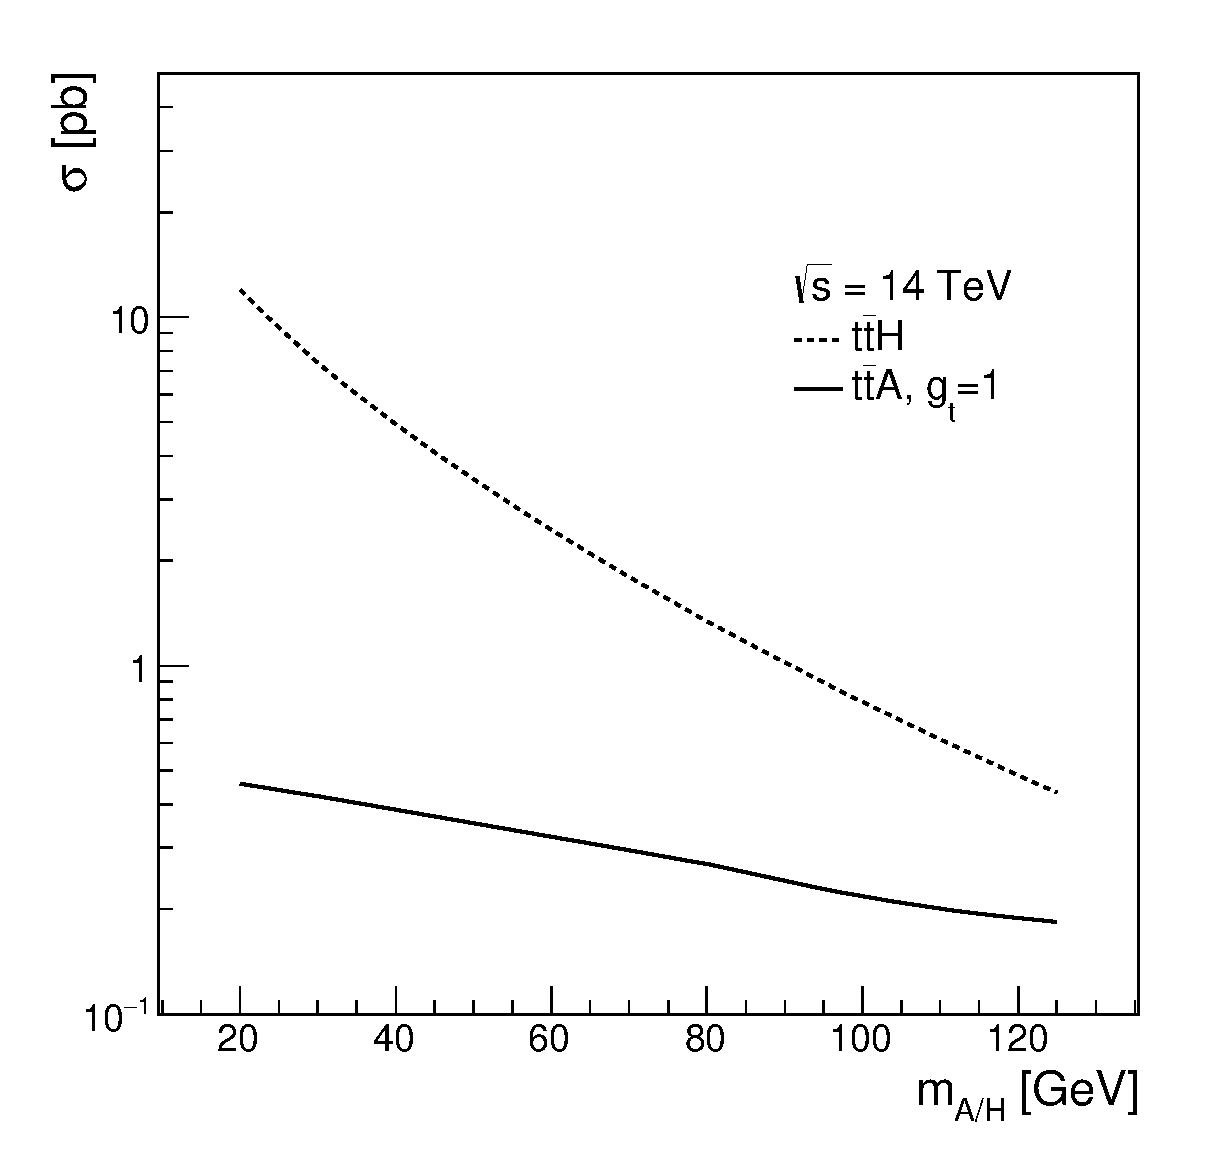
\includegraphics[width=0.4\textwidth]{Figures/XSec.eps} &
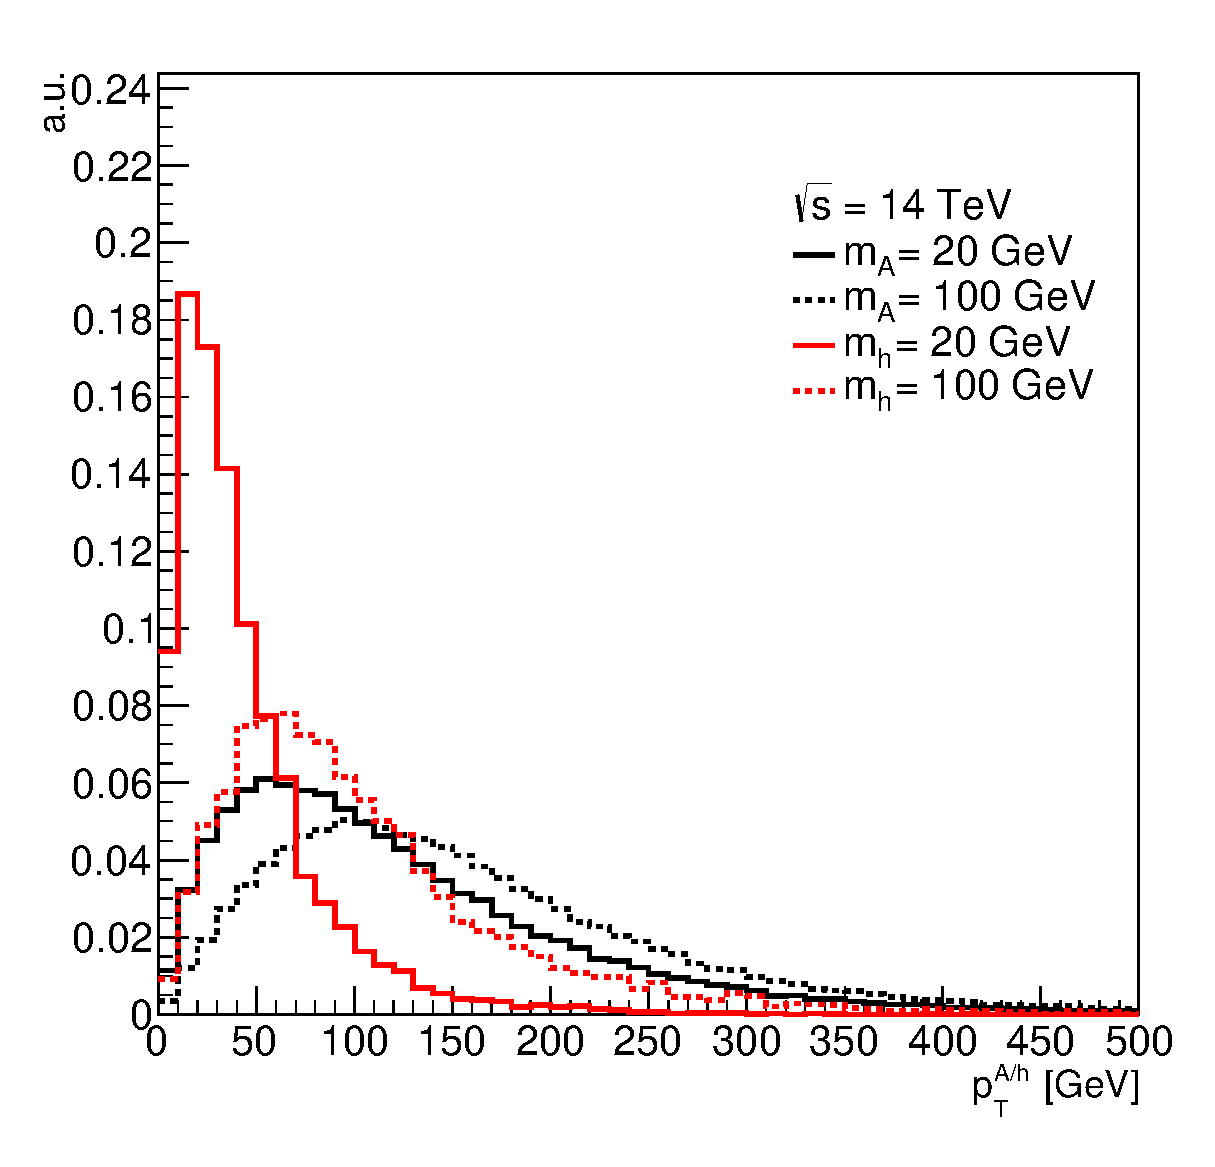
\includegraphics[width=0.4\textwidth]{Figures/hpt.eps} \\
(a) & (b) \\
\end{tabular}
\caption{\small {(a) Comparison of the leading-order cross section for $\ttbar h$ (solid line) and 
$\ttbar A$ (dashed line) in $pp$ collisions at $\sqrt{s}=14$ TeV as a function of Higgs boson mass.
In both cases a value of $g_t = 1$ is assumed. (b) Comparison of the Higgs boson $\pt$ between 
$\ttbar h$ (red) and $\ttbar A$ (black) for two different values of the Higgs boson mass, 20 GeV (solid) and 100 GeV (dashed).}}
\label{fig:xsect_pTA_ttA} 
\end{center}
\end{figure}
%%%%%%%%%%%%%%%%%%%%%%%%%%%%%%%%%%%%%%%%%%%%%%%%%% 

A large sample of $\ttbar$+jets background events is generated with up to two additional partons  in the 5F scheme 
(i.e. including $b$- and $c$-quarks). To avoid double-counting of partonic configurations generated by both the 
matrix-element  calculation and the parton shower,  a parton--jet matching scheme (``MLM matching'')~\cite{Mangano:2001xp} 
is employed. The sample is normalised to a cross section of 990 pb obtained using {\sc Top++} v2.0~\cite{Czakon:2011xx} 
at next-to-next-to-leading order (NNLO) in QCD, including resummation of next-to-next-to-leading logarithmic (NNLL) soft gluon 
terms~\cite{Cacciari:2011hy,Baernreuther:2012ws,Czakon:2012zr,Czakon:2012pz,Czakon:2013goa}, 
and using the MSTW 2008 NNLO~\cite{Martin:2009iq,Martin:2009bu} PDF set.
The $\ttbar$+jets sample is generated inclusively, but events are categorised depending
on the flavour content of additional particle jets in the event (i.e. jets not originating from
the decay of the $\ttbar$ system). Particle jets are reconstructed with the anti-$k_t$~\cite{Cacciari:2008gp,Cacciari:2005hq,Cacciari:2011ma} 
algorithm with a radius parameter $R=0.4$ and are required to have $\pt>15$~GeV and
$|\eta|<2.5$. Events where at least one such particle jet is matched within $\Delta R<0.4$ to a $b$-hadron
with $\pt>5$~GeV not originating from a top quark decay are generically labelled as $\ttbar$+$\geq$$1b$ events.
Similarly, events where at least one such particle jet is matched within $\Delta R<0.4$ to a $c$-hadron
with $\pt>5$~GeV not originating from a $W$ boson decay, and that are not labelled already as $\ttbar$+$\geq$$1b$, 
are labelled as $\ttbar$+$\geq$$1c$  events. Events labelled as either $\ttbar$+$\geq$$1b$  or
$\ttbar$+$\geq$$1c$ are generically referred to below as $\ttbar$+HF events, where HF stands for ``heavy flavour''.
We do not apply dedicated corrections to the normalisation of $\ttbar$+HF events, since Run 1 searches at the LHC~\cite{Aad:2015gra} 
showed that the LO prediction from {\sc Madgraph5} using the same settings as us is consistent with data within $\sim 20\%$,
and a larger systematic uncertainty will be assumed in this study.
As in Ref.~\cite{Aad:2015gra}, a finer categorisation of $\ttbar$+HF events is considered for the purpose of assigning systematic uncertainties
associated with the modelling of heavy-flavour production in different topologies. In this way, a distinction is
made between events with only one extra heavy-flavour jet satisfying the above cuts (referred to as $\ttbar$+$b$ or $\ttbar$+$c$),
events with two extra heavy-flavour jets (referred to as $\ttbar$+$b\bar{b}$ or $\ttbar$+$c\bar{c}$), and events
with one extra heavy-flavour jet containing two $b$- or $c$-hadrons  (referred to as $\ttbar$+$B$ or $\ttbar$+$C$).
The remaining events are labelled as $\ttbar$+light-jet events, including those with no additional jets. 

Additional background samples corresponding to $\ttbar W$, $\ttbar Z$ and $\ttbar h_{\rm SM}$ production, where $h_{\rm SM}$ is the SM Higgs boson,
are also produced. The $\ttbar W$ sample is generated requiring at least one $W$ boson in the event to decay leptonically,
and is normalised to the corresponding LO cross section, 0.404 pb, times a k-factor of 1.4~\cite{Garzelli:2012bn}.
The $\ttbar Z$ sample is generated requiring $Z \to q\bar{q}$ decays and is normalised
to the corresponding LO cross section, 0.353 pb, times a k-factor of 1.3~\cite{Garzelli:2012bn}.
Finally, the $\ttbar h_{\rm SM}$ sample is generated assuming $m_h=125$~GeV and requiring $h \to b\bar{b}$ decays.
It is normalised to the NLO cross section~\cite{Dawson:2003zu,Beenakker:2002nc,Beenakker:2001rj}, 0.611 pb, 
times the $h_{\rm SM} \to b\bar{b}$ branching ratio of 57.7\%~\cite{Djouadi:1997yw,Bredenstein:2006rh,Actis:2008ts,Denner:2011mq},
collected in Ref.~\cite{Dittmaier:2011ti}.
In these samples $Z \to q\bar{q}$ and $h_{\rm SM} \to b\bar{b}$ decays are performed by {\sc Madgraph5} and top quarks 
and $W$ bosons are decayed by {\sc Pythia}. 

\subsection{Event reconstruction}
\label{sec:event_reco}

The generated  samples at the particle level are processed through a simplified simulation of the detector
response and object reconstruction.

Isolated leptons (electrons or muons) are required to originate from a $W$ boson or $\tau$-lepton decay and
to have $\pt>25$ GeV and $|\eta|<2.5$. Furthermore, they are required to not overlap with jets, as discussed
below. A typical per-lepton identification efficiency of 80\% is assumed.

Stable particles from {\sc Pythia}, except for muons and neutrinos, are processed through a simplified
simulation of a calorimeter. The four momenta of particles falling within the same window in $\eta$--$\phi$ space of 
size $\Delta\eta \times \Delta\phi = 0.1\times 0.1$ are added together to simulate the finite granularity of
calorimeter cells. For each cell, the total three momentum is rescaled such as to make the cell massless.
Cells with energy larger than 0.1 GeV and $|\eta|<5.0$ become the inputs to the jet algorithm.
Several types of jets are considered in this analysis.

The anti-$k_t$ algorithm is used to reconstruct jets with two different radius parameters, $R=0.2$ and $R=0.4$, referred
to as AKT2 and AKT4 jets respectively. The minimum jet $\pt$ threshold for reconstruction is 5 GeV. 
During jet reconstruction, no distinction is made between identified electrons and jet energy deposits, and
so every electron is also reconstructed a jet. In order to remove this double counting, if any of the jets in the AKT2 and AKT4 collections
lie within $\Delta R=0.2$ of a selected electron, the closest jet from each jet collection is discarded.
Since this analysis has a large number of $b$-quark initiated jets, for which a significant fraction of energy
is carried away by muons in semi-muonic $b$-hadron decays, the four momenta of all reconstructed muons 
with $\pt>4$ GeV that are ghost-associated~\cite{Cacciari:2007fd,Cacciari:2008gn} to a jet are added to the calorimeter jet four momentum.
After this correction, a minimum $\pt$ requirement of 15 GeV and 25 GeV is made
for AKT2 and AKT4 jets respectively. All jets are required to satisfy $|\eta|<2.5$. 
Finally, any electron or muon within $\Delta R=0.4$ of a selected AKT4 jet is discarded.
In this analysis AKT4 jets are used to define the minimum jet multiplicity required in the event selection, while 
AKT2 jets are used to define the $b$-tag multiplicity of the event. The latter is particularly important since 
at low $m_A$ values the $b$-quarks from the $A \to b\bar{b}$ decay emerge with small angular separation.
The flavour of an AKT2 jet is determined by matching it within $\Delta R=0.15$ with a $b$-hadron or 
a $c$-hadron (not originating from a $b$-hadron decay), resulting in the jet being labelled as $b$-jet or $c$-jet respectively. 
The rest of the jets are taken to originate from the fragmentation of a light quark or gluon and are labelled 
as ``light jets". Heavy-flavour tagging is modelled in a probabilistic fashion by assigning a per-jet efficiency of 
70\% to $b$-jets, 20\% to $c$-jets, and 0.7\% to light jets.

In addition, jets are reconstructed with the Cambridge-Aachen (C/A) algorithm~\cite{Dokshitzer:1997in,Wobisch:1998wt} 
in order to reconstruct the $A \to b\bar{b}$ decay, taking advantage of the boost with which $A$ bosons are produced in the
$\ttbar A$ process. Two radius parameters are considered for C/A jets, $R^{\rm C/A}=0.6$ and 0.8, referred to as CA6 and CA8 jets 
respectively. The choice of radius for C/A jets is optimised in order to optimally
reconstruct the $\ttbar A$ signal depending on the value of $m_A$. In order to minimise the impact of
soft radiation and pileup (not modelled in this analysis), the mass-drop (a.k.a. BDRS) filtering algorithm~\cite{Butterworth:2008iy, Plehn:2009rk} 
with the following parameters, $\mu_{\rm frac}=0.67$ and $y_{\rm cut}=0.09$~\cite{Aad:2013gja}, is applied to the
reconstructed C/A jets. A semi-muonic energy correction to the C/A jet four momentum is also applied, as in the case of AKT2 and AKT4 jets.

